\mia{Will move stuff down to discussion, but simpler to write in the same section for now}

\subsubsection{Franke function}

\begin{figure}
    \centering
    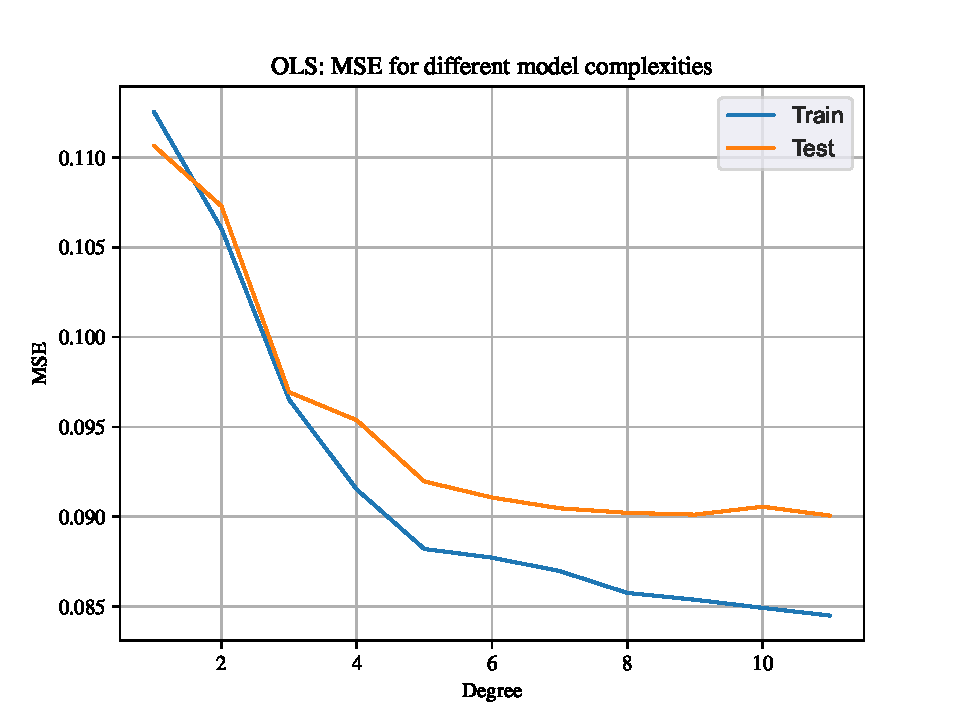
\includegraphics[width=1\linewidth]{project_1_alt/figures/data/OLS_MSE_Franke_Noise.pdf}
    \caption{Caption}
    \label{fig:mseols}
\end{figure}

Fig. \ref{fig:mseols} shows how the error initially decreases as the degree of complexity increases. This seems reasonable as the Franke function makes up a complicated surface and one would think that higher degree polynomials are necessary to replicate it. 

We furthermore notice how at around degree = 9, the test error reaches its minimum. The error increases as the polynomial degree is increased by one. We use the test error to choose the optimal degree of complexity. In this case, polynomials of degree up to nine is the best. The training error continues to decrease. This is due to overfitting and the fact that OLS is designed to minimize the MSE. 

%At around degree = 11, the MSE for both the training and test data set increases substantially. This may initially seem wrong. The OLS is inherently designed to minimize MSE and in theory, we would expect it to continue to decrease infinitely. The problem we encounter here is numerical precision. At this point we look at very small numbers to the power of 12. This becomes numbers smaller than $10^{15}$, the numbers we can represent on our computers. 

\begin{figure}
    \centering
    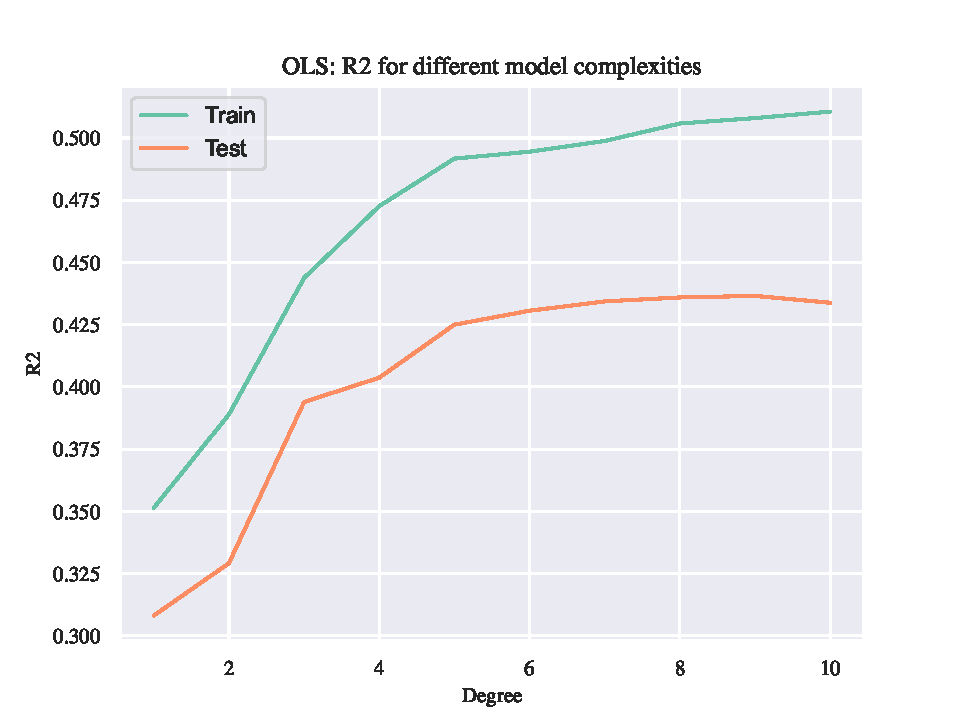
\includegraphics[width=1\linewidth]{project_1_alt/figures/data/OLS_R2_Franke_Noise.pdf}
    \caption{Caption}
    \label{fig:r2ols}
\end{figure}

$R^2$ \mia{more more}

\begin{figure}
    \centering
    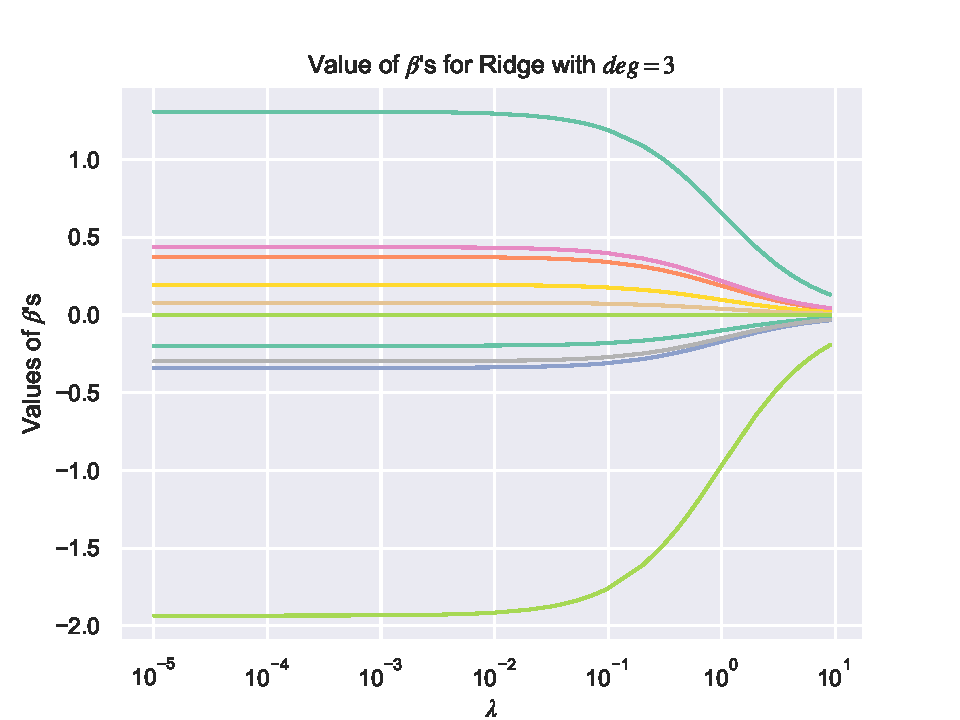
\includegraphics[width=1\linewidth]{project_1_alt/figures/data/Ridge_Betas_lambda_Franke_Noise_const_deg.pdf}
    \caption{\mia{Caption}}
    \label{fig:ridge_betas}
\end{figure}

\begin{figure}
    \centering
    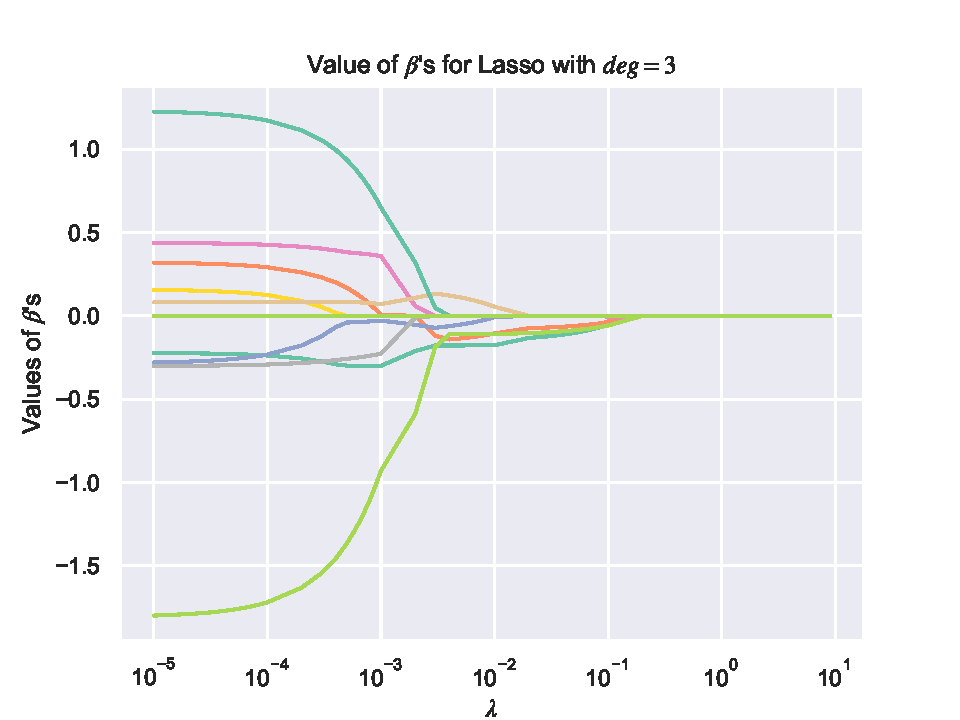
\includegraphics[width=1\linewidth]{project_1_alt/figures/data/Lasso_Betas_lambda_Franke_Noise_const_deg.pdf}
    \caption{\mia{caption}}
    \label{fig:lasso_betas}
\end{figure}

The $\beta$'s values for our Ridge- and Lasso regression models are presented in fig. \ref{fig:ridge_betas} and fig. \ref{fig:lasso_betas} respectfully. For both models, we observe that the values of the coefficients are forced towards zero, and thereby also each other, as the penalty increases. For the Ridge regression coefficients, all have non-zero values regardless of the size of the penalty. For Lasso regression however, we observe that some are brought to zero at a sufficiently large penalty. Both dark blue lines are at a zero value at approximately $\lambda = 10^0 = 1$, while all but yellow and purple have reached zero when $\lambda \approx 10$. 

\begin{figure}[h!]
    \centering
    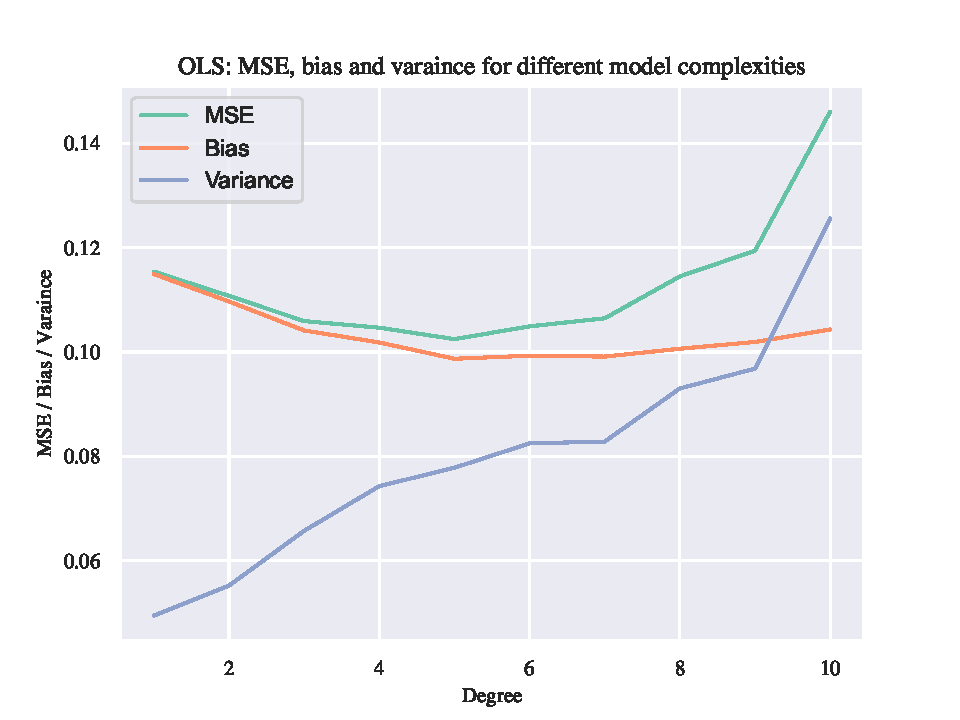
\includegraphics[width=1\linewidth]{project_1_alt/figures/data/bias_var_Franke_Noise_bootstrap.pdf}
    \caption{caption}
    \label{bias_var_trade}
\end{figure}

For the OLS model trained with bootstrapping, fig. \ref{bias_var_trade} shows how the MSE can be decomposed into a bias and variance term. 

\begin{figure}[h!]
    \centering
    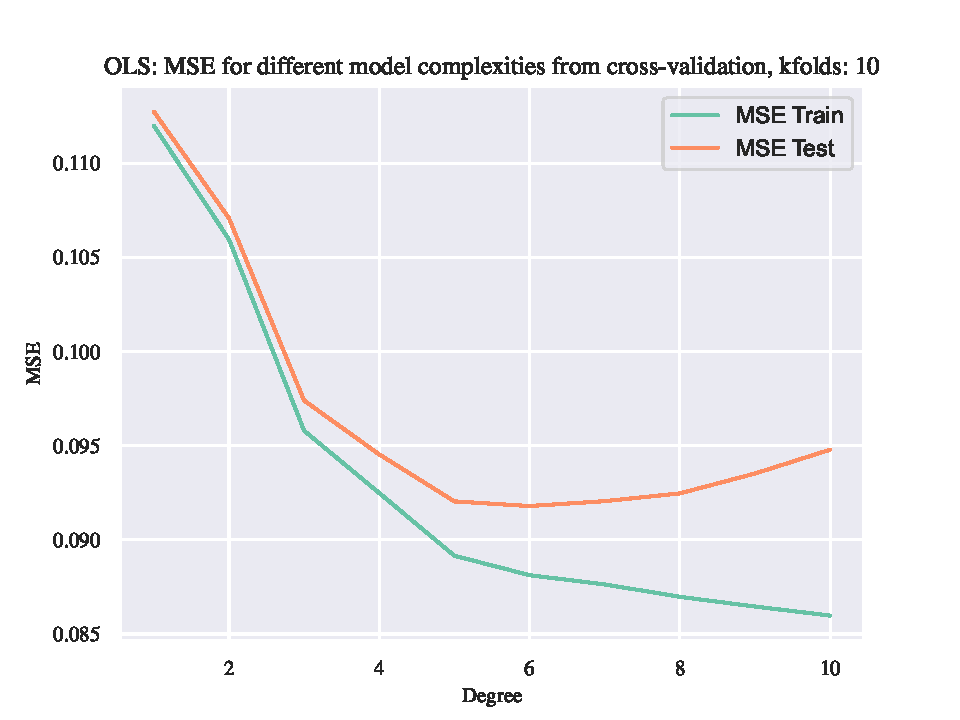
\includegraphics[width=1\linewidth]{project_1_alt/figures/data/OLS_MSE_Franke_Noise_CV_k10.pdf}
    \caption{Caption}
    \label{fig:frankek10}
\end{figure}

\mia{more more}

\mia{cv versus bootstrap}

\begin{figure}
    \centering
    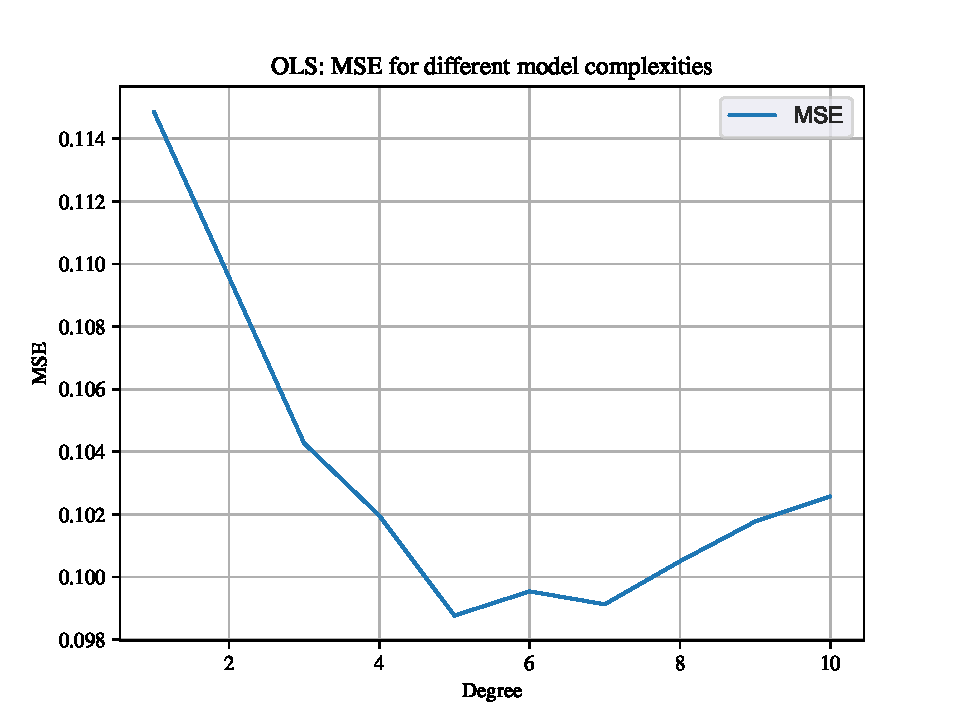
\includegraphics[width=1\linewidth]{project_1_alt/figures/data/OLS_MSE_Franke_Noise_bootstrap.pdf}
    \caption{Caption}
    \label{fig:olsfrankebootstrap}
\end{figure}

\begin{figure}
    \centering
    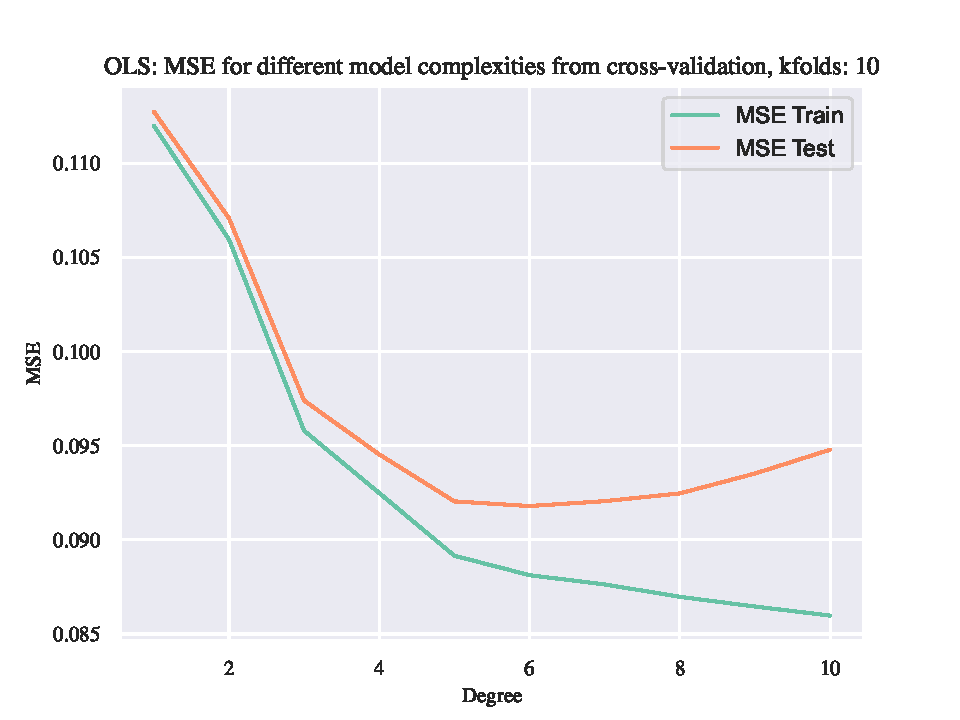
\includegraphics[width=1\linewidth]{project_1_alt/figures/data/OLS_MSE_Franke_Noise_CV_k10.pdf}
    \caption{Caption}
    \label{fig:cvk10franke}
\end{figure}

\subsubsection{Terrain data function}



\plothere{OLS, Ridge and Lasso for terrain data}

\plothere{OLS, Ridge and Lasso for terrain data with CV}

\plothere{OLS, Ridge and Lasso for terrain data with bootstrap}


